\section{Framework}

O framework aqui apresentado foi originalmente proposto por \cite{aloupis2015classic}, e tem
como objetivo provar a NP-Hardness de jogos de plataforma. Para isso, ele implementa diversos dispositivos.
Apesar de The Legend of Zelda: a Link to The Past não ser um jogo de plataforma, mostraremos como ele se encaixa neste modelo.

\begin{figure}[!htb]
     \centering
     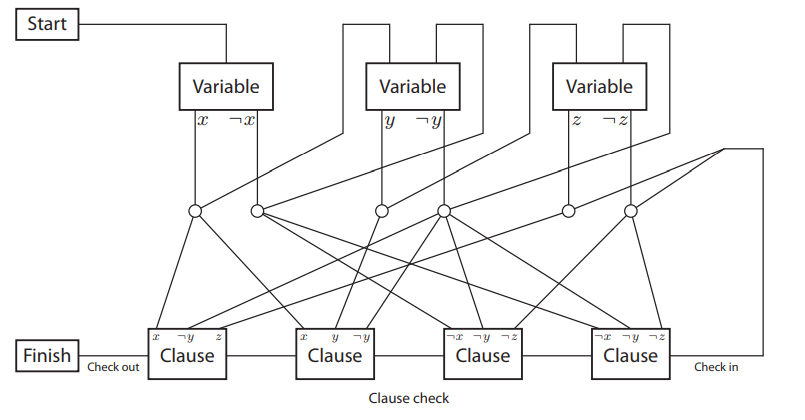
\includegraphics[scale=0.5]{framework.png}
     \caption{Framework geral para prova da NP Completude}
\end{figure}

Essa framework funciona da seguinte maneira: O jogador começa na posição Start. 
Cada dispositivo de variável obriga o jogador a fazer uma escolha
exclusiva de "verdadeiro" (\(x\)) ou "falso" (\(\lnot x\)) como valor para a variável para uma fórmula booleana. Ambas as escolhas
permitem ao jogador seguir caminhos que levam aos dispositivos de Cláusula, correspondentes as clausulas
que contém aquela literal (\(x\) ou \(\lnot x\)). Esses caminhos podem se cruzar, mas o dispositivo de Crossover
previne que o jogador troque entre caminhos cruzados. Ao visitar o dispositivo de cláusula, o jogador pode
desbloquear a cláusula (um estado permanente de mudança), mas não pode alcançar nenhum dos outros caminhos
conectados ao dispositivo de cláusula. Por fim, depois de atravessar através de todos os dispositivos de variáveis,
chegará a posição final. O jogador pode passear o caminho de checagem se e somente se cada cláusula for desbloqueada
por algum literal. Portanto, basta implementar os dispositivos citados para provar a NP-Hardness de qualquer jogo de plataforma.

Os dispositivos devem seguir as seguintes propriedades:

\textbf{Começo e Fim: } Os dispositivos de começo e fim contém o ponto inicial e o objetivo do personagem, respectivamente.

\textbf{Variável: }Cada dispositivo de variável precisa forçar o jogador a escolher um entre dois caminhos, correspondendo
a (\(xi\)) ou sua negação \(\lnot xi\) sendo escolhidos como o literal satisfeito, como por exemplo o caminho que foi escolhido ou o
caminho que não pode ser transposto. Cada dispositivo de variável deve ser acessível por apenas e tão somente o dispositivo de 
variável anterior, independentemente da escolha feita no dispositivo anterior, no qual o caminho a entrada de um literal não
permita a travessia de volta para a negação do literal.

\textbf{Cláusula e Checagem: }Cada dispositivo de cláusula deve ser acessível do (e inicialmente, apenas do) caminho vindo do
literal correspondente aos literais que aparecem na cláusula da fórmula Booleana. Além disso, quando um jogador
visita o dispositivo de cláusula dessa maneira, ele deve realizar alguma ação que "destrave" o dispositivo. O caminho de checagem
atravessa todo dispositivo de cláusula em sequência, e o jogador pode passar em todos os dispositivos de cláusula através do 
caminho de checagem se e apenas se o dispositivo de cláusula estiver desbloqueado. Assim o caminho de verificação pode ser
totalmente atravessado apenas se todos os dispositivos de variável tiverem sido visitadas dos caminhos de literais. Se o jogador
atravessar todo o caminho de verificação, ele pode acessar o dispositivo de fim.

\textbf{Crossover: }O dispositivo Crossover deve permitir a travessia através de duas passagens que se cruzam,
de tal forma que não há vazamento entre elas.
